% Uncomment this line for on-screen presentation
\documentclass[xcolor={dvipsnames}]{beamer}\usepackage{etoolbox}\newtoggle{printable}\togglefalse{printable}

% Uncomment this line for printable slides (disable animations and don't waste ink)
%\documentclass[handout, xcolor={dvipsnames}]{beamer}\usepackage{etoolbox}\newtoggle{printable}\toggletrue{printable}

% Adjust these for the path of the theme and its graphics, relative to this file
%\usepackage{beamerthemeFalmouthGamesAcademy}
\usepackage{../../beamerthemeFalmouthGamesAcademy}
\graphicspath{ {../../} }

% Default language for code listings
\lstset{language=C++,
		morekeywords={each,in}
}

\begin{document}
\title{Programming Practice VI}   
\subtitle{BSc Computing for Games}

\frame{\titlepage} 

\part{Morning}
\frame{\partpage}

\begin{frame}{Agile Principles}
	In the morning session you will:
	
	\begin{itemize}
		\item \textbf{Prepare} the group presentation for the Agile report.
		\begin{itemize}
			\item Each member of the group must have a different research question and have it approved by a tutor.
			\item Collaborate on research activities, such as recommending source material.
			\item Engage in peer review.
			\item Create the slides as a group. Try to allocate the same number of slides to each member of the group.
		\end{itemize}
		\item \textbf{Practice} your group presentation.
	\end{itemize}
\end{frame}

\part{Afternoon}
\frame{\partpage}

\begin{frame}{Collaborative Project}
	In the afternoon session you will:
	
	\begin{itemize}
		\item Continue working on the game.
		\item \textbf{Prepare} the product backlog on the Trello board.
		\item \textbf{Conduct} a Sprint Planning meeting with your COMP150 group.
	\end{itemize}
\end{frame}

% -------------------------------------------------------

%\part{The compiler}
%\frame{\partpage}
%
%\begin{frame}
%	\frametitle{The build process}
%	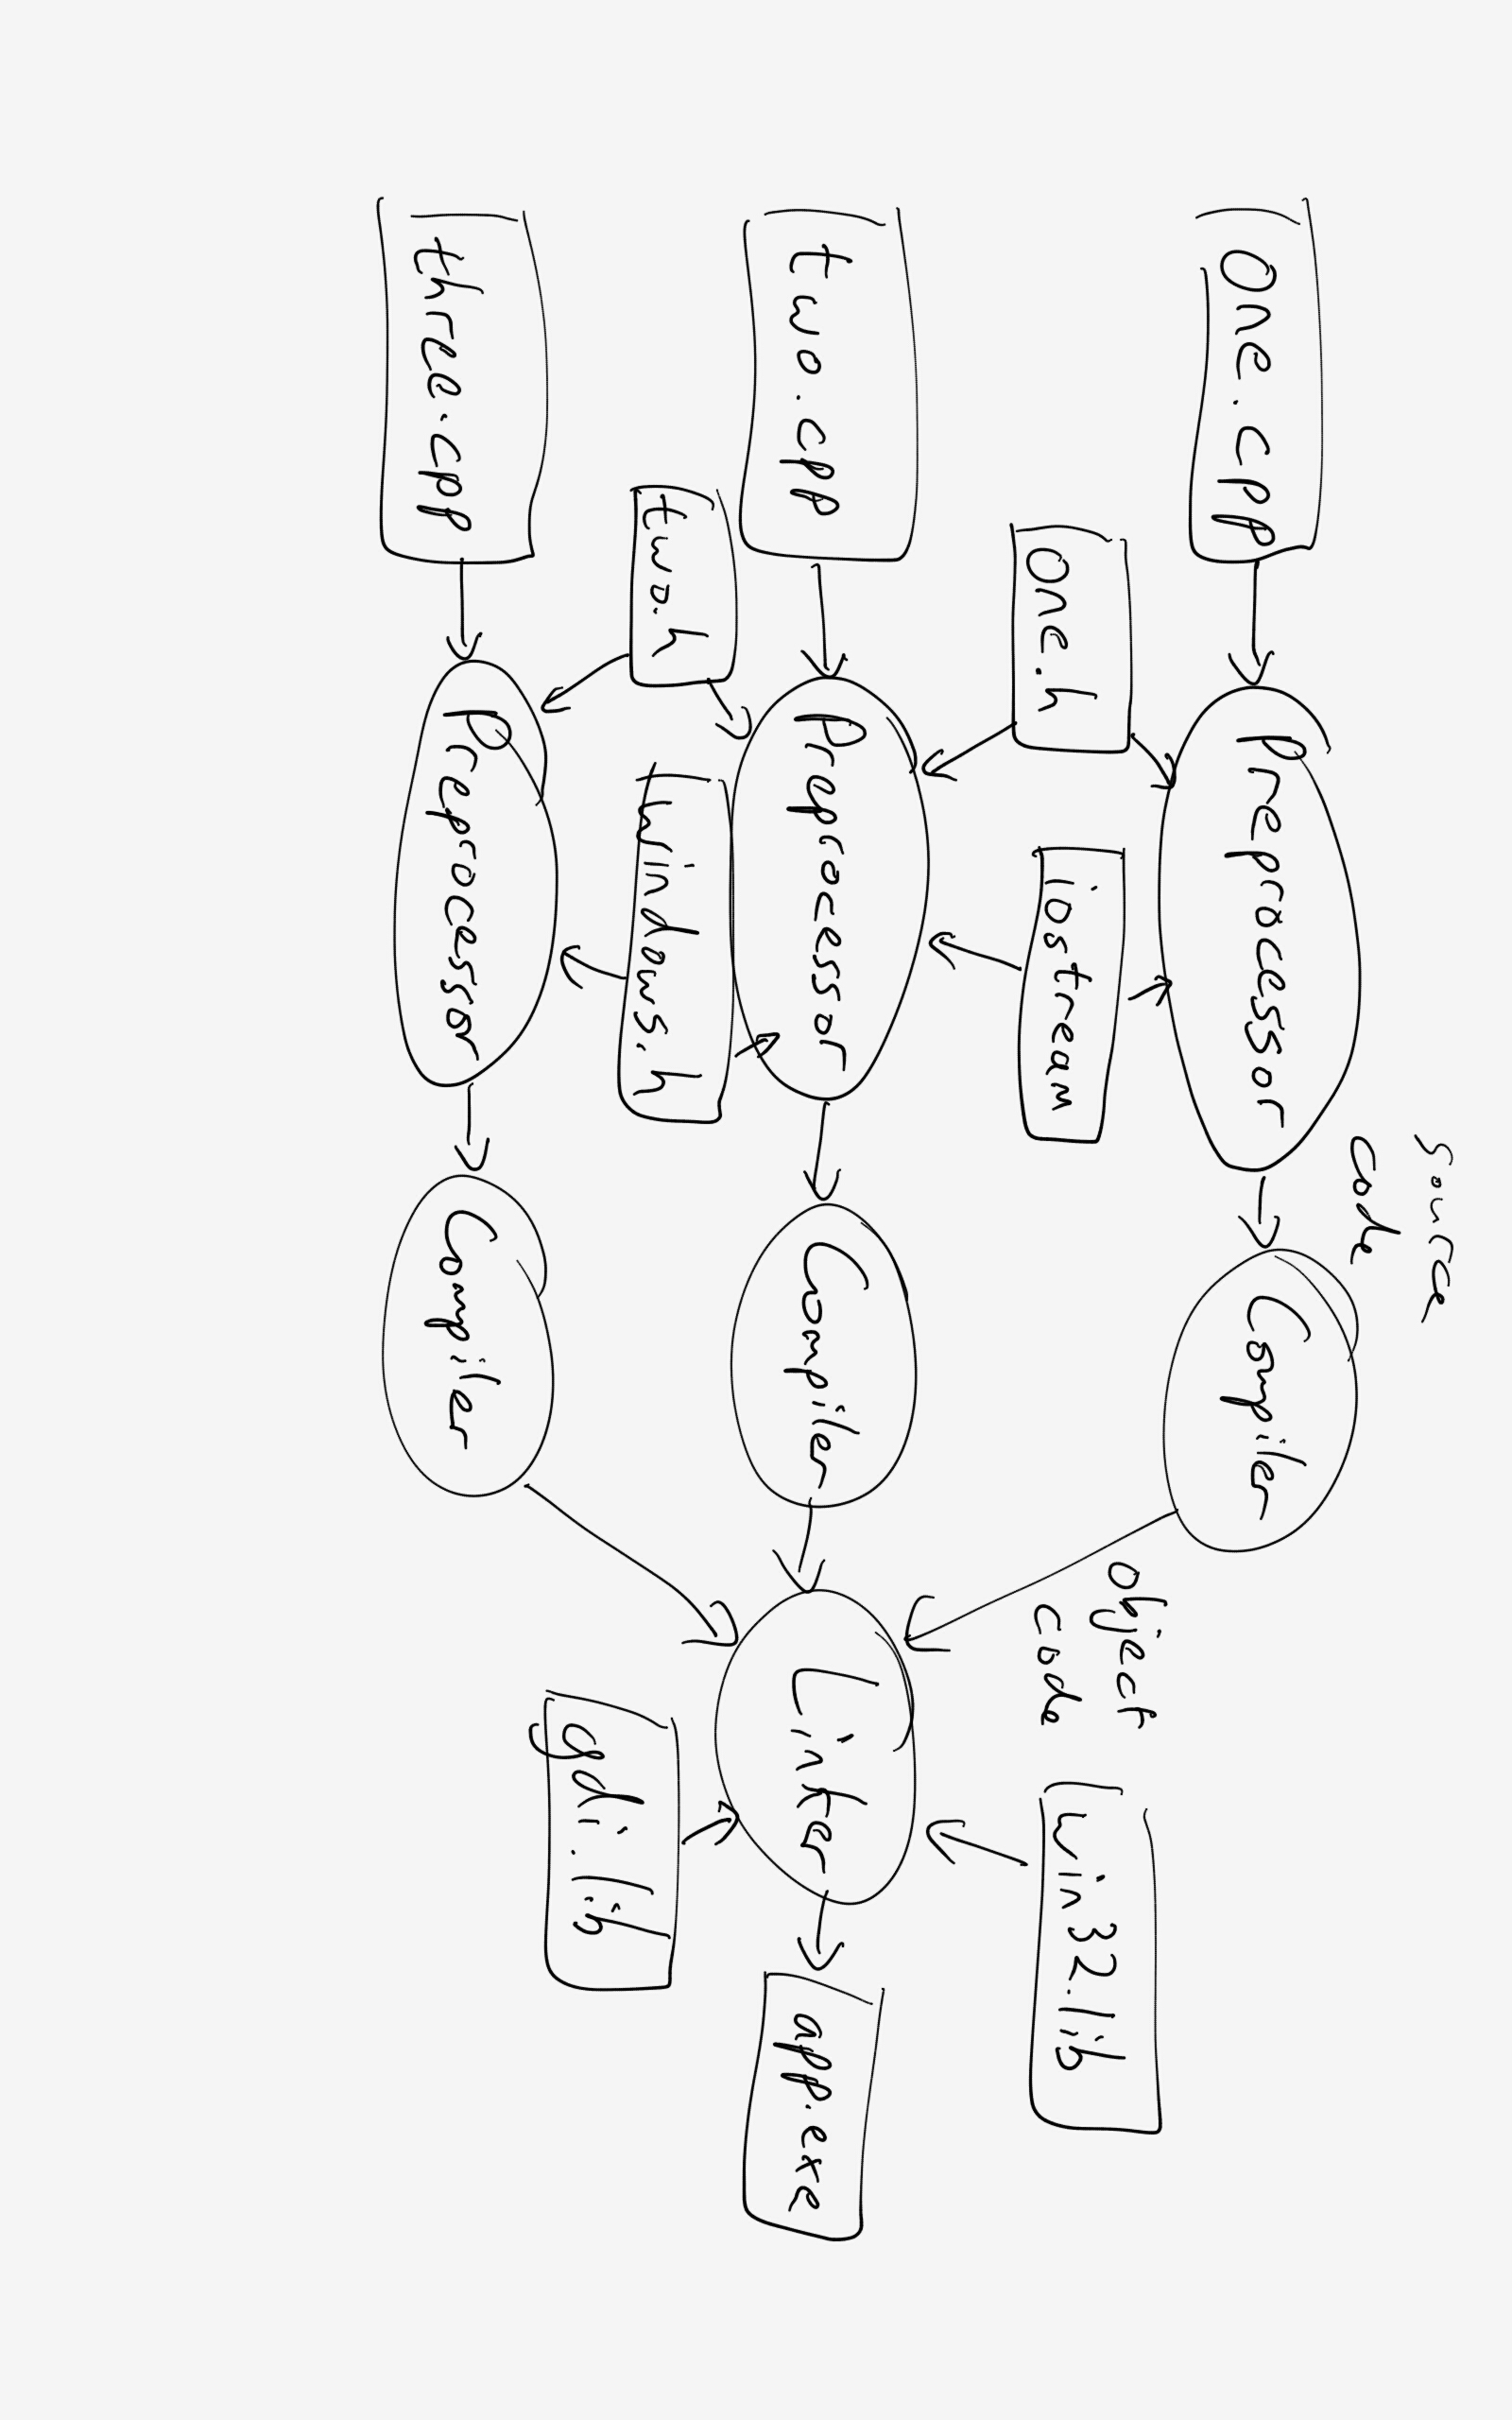
\includegraphics[height=\textwidth,angle=90]{compiler_sketch}
%\end{frame}

\end{document}
